\documentclass[10pt, a4paper]{article}

% \usepackage[mathdisplays=normal]{savetrees}

% Core packages for better typography
\usepackage[utf8]{inputenc}
\usepackage[T1]{fontenc}
\usepackage{microtype}
\usepackage{lmodern}
\usepackage{setspace}
% \onehalfspacing

% Math packages with better formatting
\usepackage{latexsym,amsfonts,amssymb,amsthm,amsmath}
\usepackage{mathtools}

% Graphics and figures
\usepackage{tikz}
\usetikzlibrary{angles,quotes}
\usepackage{pgfplots}
\pgfplotsset{compat=newest}
\usepackage{graphicx}
\graphicspath{{../data/}}

% Better table formatting
\usepackage{booktabs}
\usepackage{array}
\usepackage{multirow}

% Force figures to stay in their sections
\usepackage[section]{placeins}
\makeatletter
\AtBeginDocument{%
  \expandafter\renewcommand\expandafter\subsection\expandafter{%
    \expandafter\@fb@secFB\subsection
  }%
}
\makeatother

% Code listing formatting
\usepackage{listings}
\usepackage{xcolor}
\definecolor{codegreen}{rgb}{0,0.6,0}
\definecolor{codegray}{rgb}{0.5,0.5,0.5}
\definecolor{codepurple}{rgb}{0.58,0,0.82}
\definecolor{backcolour}{rgb}{0.95,0.95,0.92}
\lstdefinestyle{mystyle}{
  backgroundcolor=\color{backcolour},   
  commentstyle=\color{codegreen},
  keywordstyle=\color{blue},
  numberstyle=\tiny\color{codegray},
  stringstyle=\color{codepurple},
  basicstyle=\ttfamily\footnotesize,
  breakatwhitespace=false,         
  breaklines=true,                 
  captionpos=b,                    
  keepspaces=true,                 
  showspaces=false,                
  showstringspaces=false,
  showtabs=false,                  
  tabsize=2
}
\lstset{style=mystyle}

% References and hyperlinks
\usepackage{pdfpages}
\usepackage[colorlinks=true, linkcolor=blue, citecolor=blue]{hyperref}
\usepackage{caption}
\usepackage{subcaption}
\usepackage{csquotes}
\usepackage[notes, backend=bibtex]{biblatex-chicago}
\addbibresource{refs.bib}

% Custom theorem environments
\newtheorem{theorem}{Theorem}[section]
\newtheorem{lemma}[theorem]{Lemma}
\newtheorem{proposition}[theorem]{Proposition}
\newtheorem{corollary}[theorem]{Corollary}
\newtheorem{definition}{Definition}[section]
\newtheorem{example}{Example}[section]

\title{\Large \bfseries SB4: Integrated Photonics\\[0.5em] \large Report}
\author{Lucas Ng\thanks{ln373@cam.ac.uk}}
\date{18th May 2025}

\begin{document}
\maketitle

\section{Modal analysis of a symmetric planar waveguide (SPW)}
This section details the analysis of symmetric planar waveguides (SPWs), focusing on silicon-on-insulator (SOI) platforms and comparisons with other material systems. All simulations and plotting were performed using MATLAB. I implemented a helper MATLAB package called \texttt{sb4} to include functionalities for obtaining material refractive indices (\texttt{sb4.get\_n}) and for planar waveguide mode analysis (\texttt{sb4.planar.find\_num\_modes}, \texttt{sb4.planar.find\_neff}).

\subsection{Silicon-on-Insulator (SOI) waveguide}
The SOI platform, consisting of a silicon (Si) core and silicon dioxide (SiO$_2$) cladding, is a prevalent choice for integrated photonics due to its high index contrast and compatibility with CMOS manufacturing.

\paragraph{Initial Mode Check at 300 nm Core}
A symmetric SOI planar waveguide with a core thickness of 300~nm, operating at a wavelength ($\lambda$) of 1550~nm, was first analyzed. The refractive index of Si ($n_{\text{Si}}$) and SiO$_2$ ($n_{\text{SiO}_2}$) at this wavelength were determined. Since \texttt{sb4.planar.find\_num\_modes} returned 2 for the first element, TE$_0$ and TE$_1$ should be supported (and hence TM$_0$ and TM$_1$ also).

Internally, this function checks the cutoff condition for planar waveguides, which is given by the following equation:

\begin{equation}
    \Delta n = n_{\text{core}} - n_{\text{clad}} > \frac{m^2\lambda^2}{4t^2(n_{\text{core}}+ n_{\text{clad}})},
\end{equation}
Here, $n_{\text{core}}$ and $n_{\text{clad}}$ are the refractive indices of the core and cladding, respectively, $\lambda$ is the wavelength, $m$ is the mode number and $t$ is the core thickness.

\paragraph{Mode Count vs. Core Thickness}
The number of supported modes was investigated as a function of the Si core thickness, swept from 200~nm to 1~{\textmu}m in increments of 100~nm, at $\lambda = 1550$~nm. As shown in Figure~\ref{fig:modes_vs_thickness_SOI_1550nm}, the number of supported modes increases with core thickness. This is expected, as a thicker core allows for more spatial variations of the electromagnetic field, accommodating higher-order modes.

\begin{figure}[h!]
    \centering
    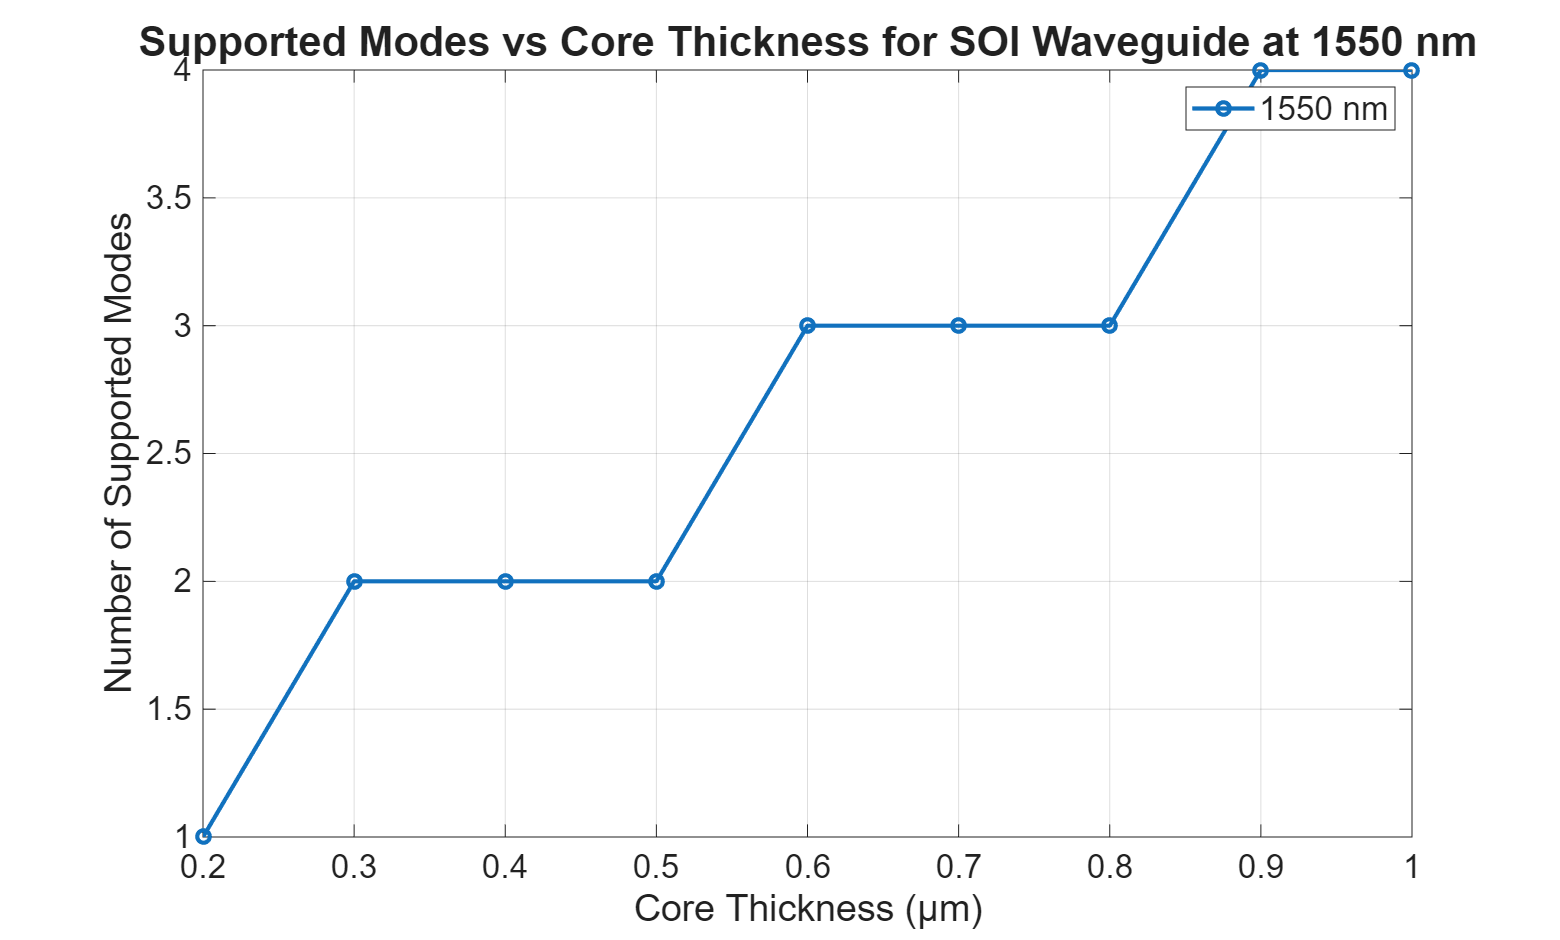
\includegraphics[width=0.8\textwidth]{task1/modes_vs_thickness_SOI_1550nm.png}
    \caption{Number of supported modes as a function of core thickness for an SOI waveguide at $\lambda = 1550$~nm.}
    \label{fig:modes_vs_thickness_SOI_1550nm}
\end{figure}

\paragraph{Mode Count vs. Wavelength}
The analysis was repeated for various operating wavelengths (850~nm, 1310~nm, 1550~nm, 1600~nm, 2000~nm), considering material dispersion. Figure~\ref{fig:modes_vs_thickness_SOI_wavelengths} illustrates that for a fixed core thickness, the number of supported modes generally decreases with increasing wavelength. This is because the mode confinement weakens at longer wavelengths relative to the waveguide dimensions, and the effective index contrast reduces.

\begin{figure}[h!]
    \centering
    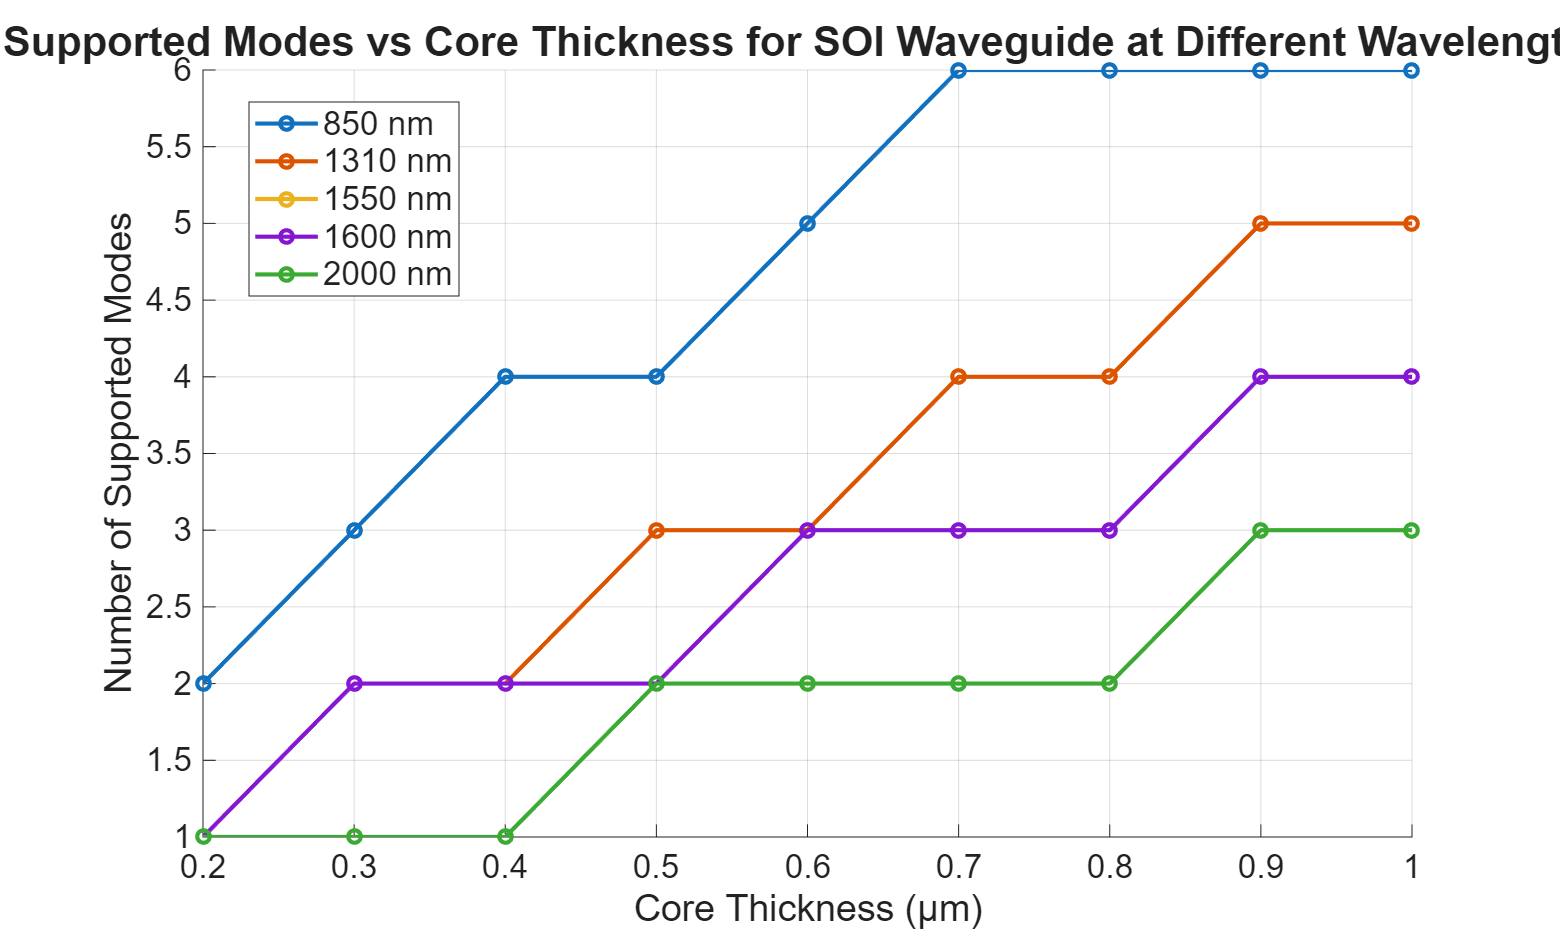
\includegraphics[width=0.8\textwidth]{task1/modes_vs_thickness_SOI_wavelengths.png}
    \caption{Number of supported modes vs. core thickness for an SOI waveguide at different operating wavelengths.}
    \label{fig:modes_vs_thickness_SOI_wavelengths}
\end{figure}

\paragraph{Effective Index Dispersion}
The effective refractive index ($n_{\text{eff}}$) of TE and TM modes was calculated as a function of core thickness (10~nm to 2~{\textmu}m) for an SOI waveguide at $\lambda = 1550$~nm. Figure~\ref{fig:neff_vs_thickness_Si_SiO2_1550nm} shows these dispersion curves. For each mode, $n_{\text{eff}}$ starts near $n_{\text{SiO}_2}$ at its cutoff thickness and increases towards $n_{\text{Si}}$ as the core thickness grows. Higher-order modes appear at progressively larger core thicknesses. The solver's ability to precisely match theoretical cutoffs can be challenging where $\nabla n_{\text{eff}}$ is small, which is why the modes on this plot appear at slightly larger core thicknesses than the theoretical critical thicknesses.

\begin{figure}[h!]
    \centering
    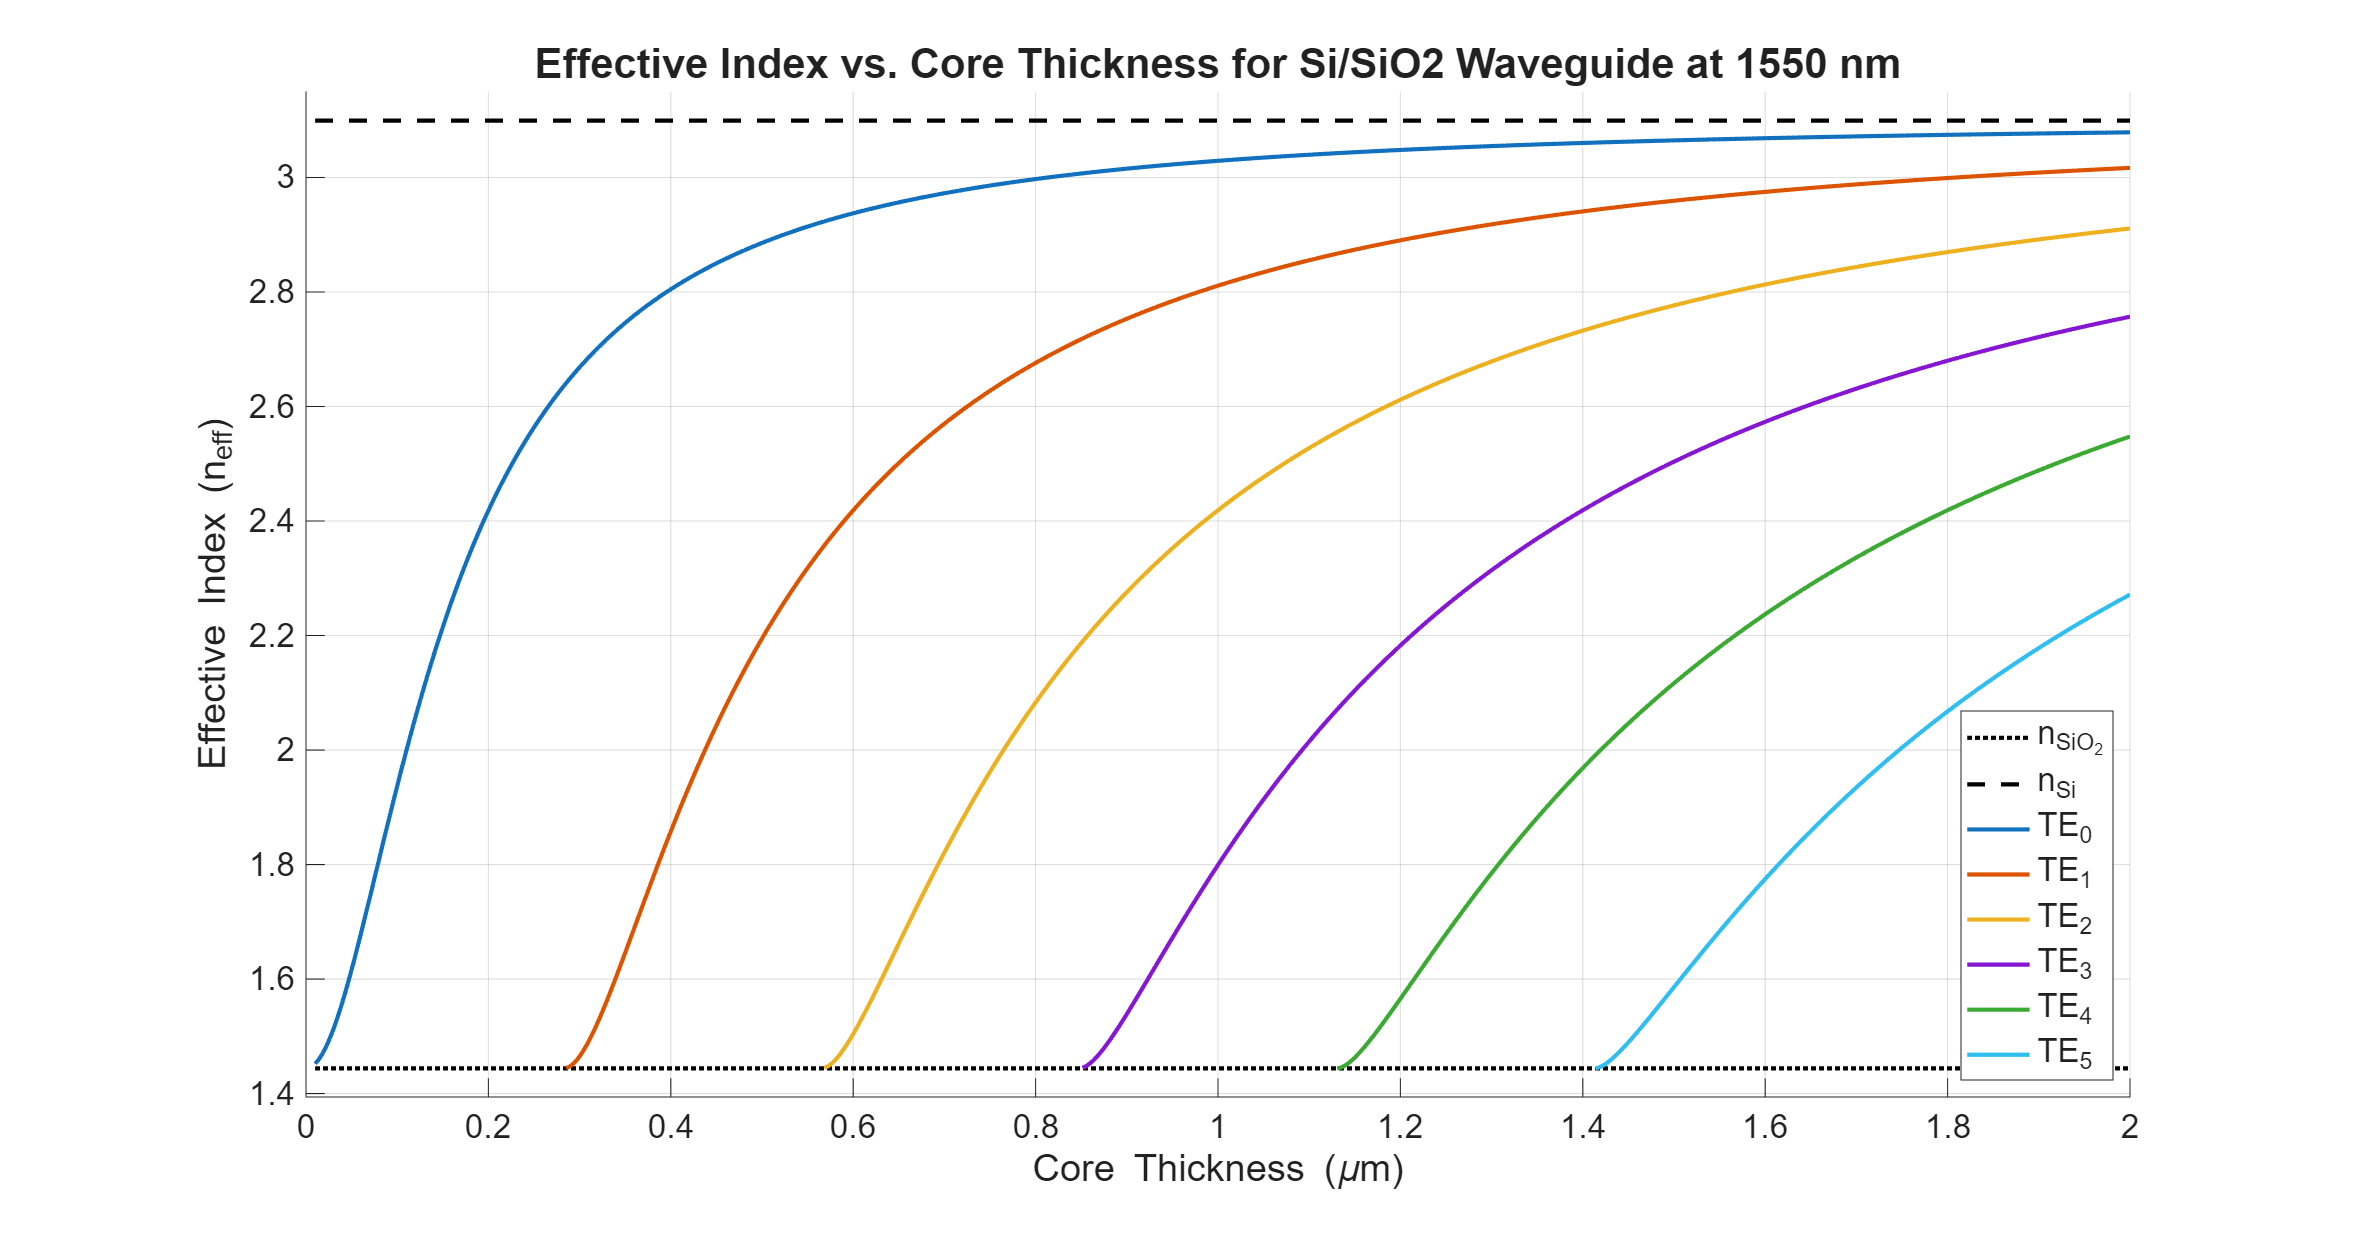
\includegraphics[width=0.8\textwidth]{task1/neff_vs_thickness_Si_SiO2_1550nm.png}
    \caption{Effective index ($n_{\text{eff}}$) vs. core thickness for TE and TM modes in an Si/SiO$_2$ waveguide at $\lambda = 1550$~nm. Horizontal lines indicate $n_{\text{Si}}$ and $n_{\text{SiO}_2}$.}
    \label{fig:neff_vs_thickness_Si_SiO2_1550nm}
\end{figure}

\paragraph{Critical Thickness for Mode Cutoff}
The theoretical critical core thickness ($t_c$) required to support a mode of order $m$ is given by $t_c = (m \lambda) / (2 \sqrt{n_{\text{core}}^2 - n_{\text{clad}}^2})$. Figure~\ref{fig:critical_thickness_vs_wavelength} plots $t_c$ against wavelength for mode orders $m=0$ to $m=4$ in an SOI waveguide. The fundamental mode ($m=0$) has no cutoff thickness. For higher-order modes, $t_c$ increases with both mode order and wavelength, reflecting the need for larger dimensions to guide less confined or longer-wavelength light.

\begin{figure}[h!]
    \centering
    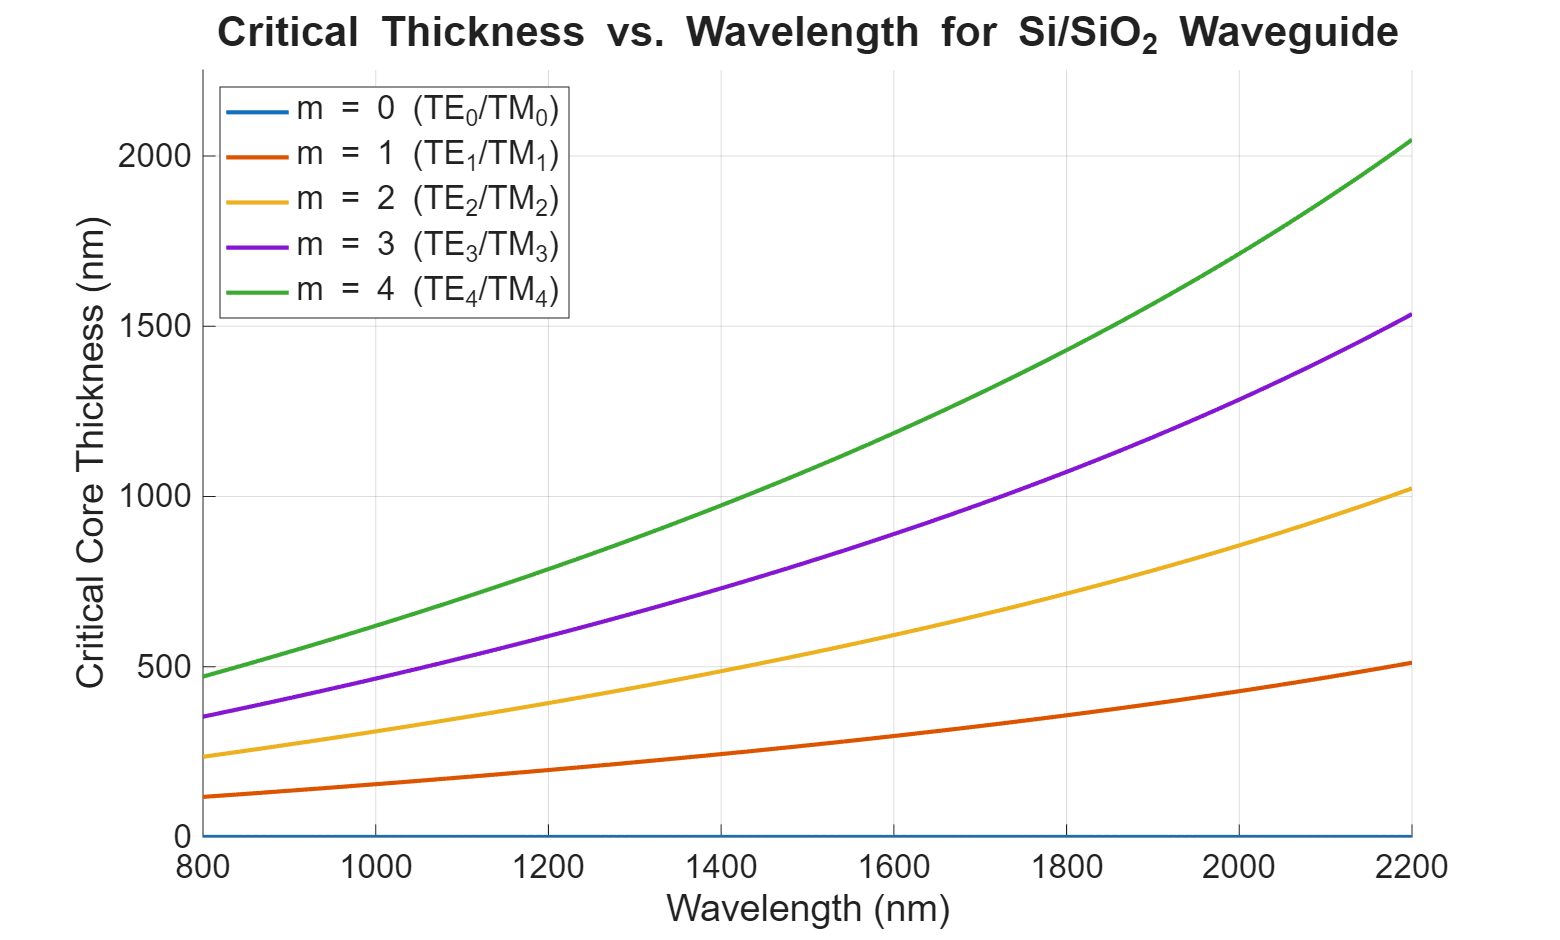
\includegraphics[width=0.8\textwidth]{task1/critical_thickness_vs_wavelength.png}
    \caption{Critical core thickness vs. wavelength for different mode orders ($m$) in an Si/SiO$_2$ waveguide.}
    \label{fig:critical_thickness_vs_wavelength}
\end{figure}

\paragraph{Group Index Dispersion}
The group index ($n_g = n_{\text{eff}} - \lambda \frac{\mathrm{d}n_{\text{eff}}}{\mathrm{d}\lambda}$) characterizes how the envelope of a light pulse propagates. Figure~\ref{fig:group_index_TE0_TM0_vs_wavelength} shows $n_g$ for the fundamental TE$_0$ and TM$_0$ modes in an SOI waveguide with a 300~nm core thickness. The group index is wavelength-dependent due to both material and waveguide dispersion, and is critical for understanding phenomena like pulse broadening.


\begin{figure}[h!]
    \centering
    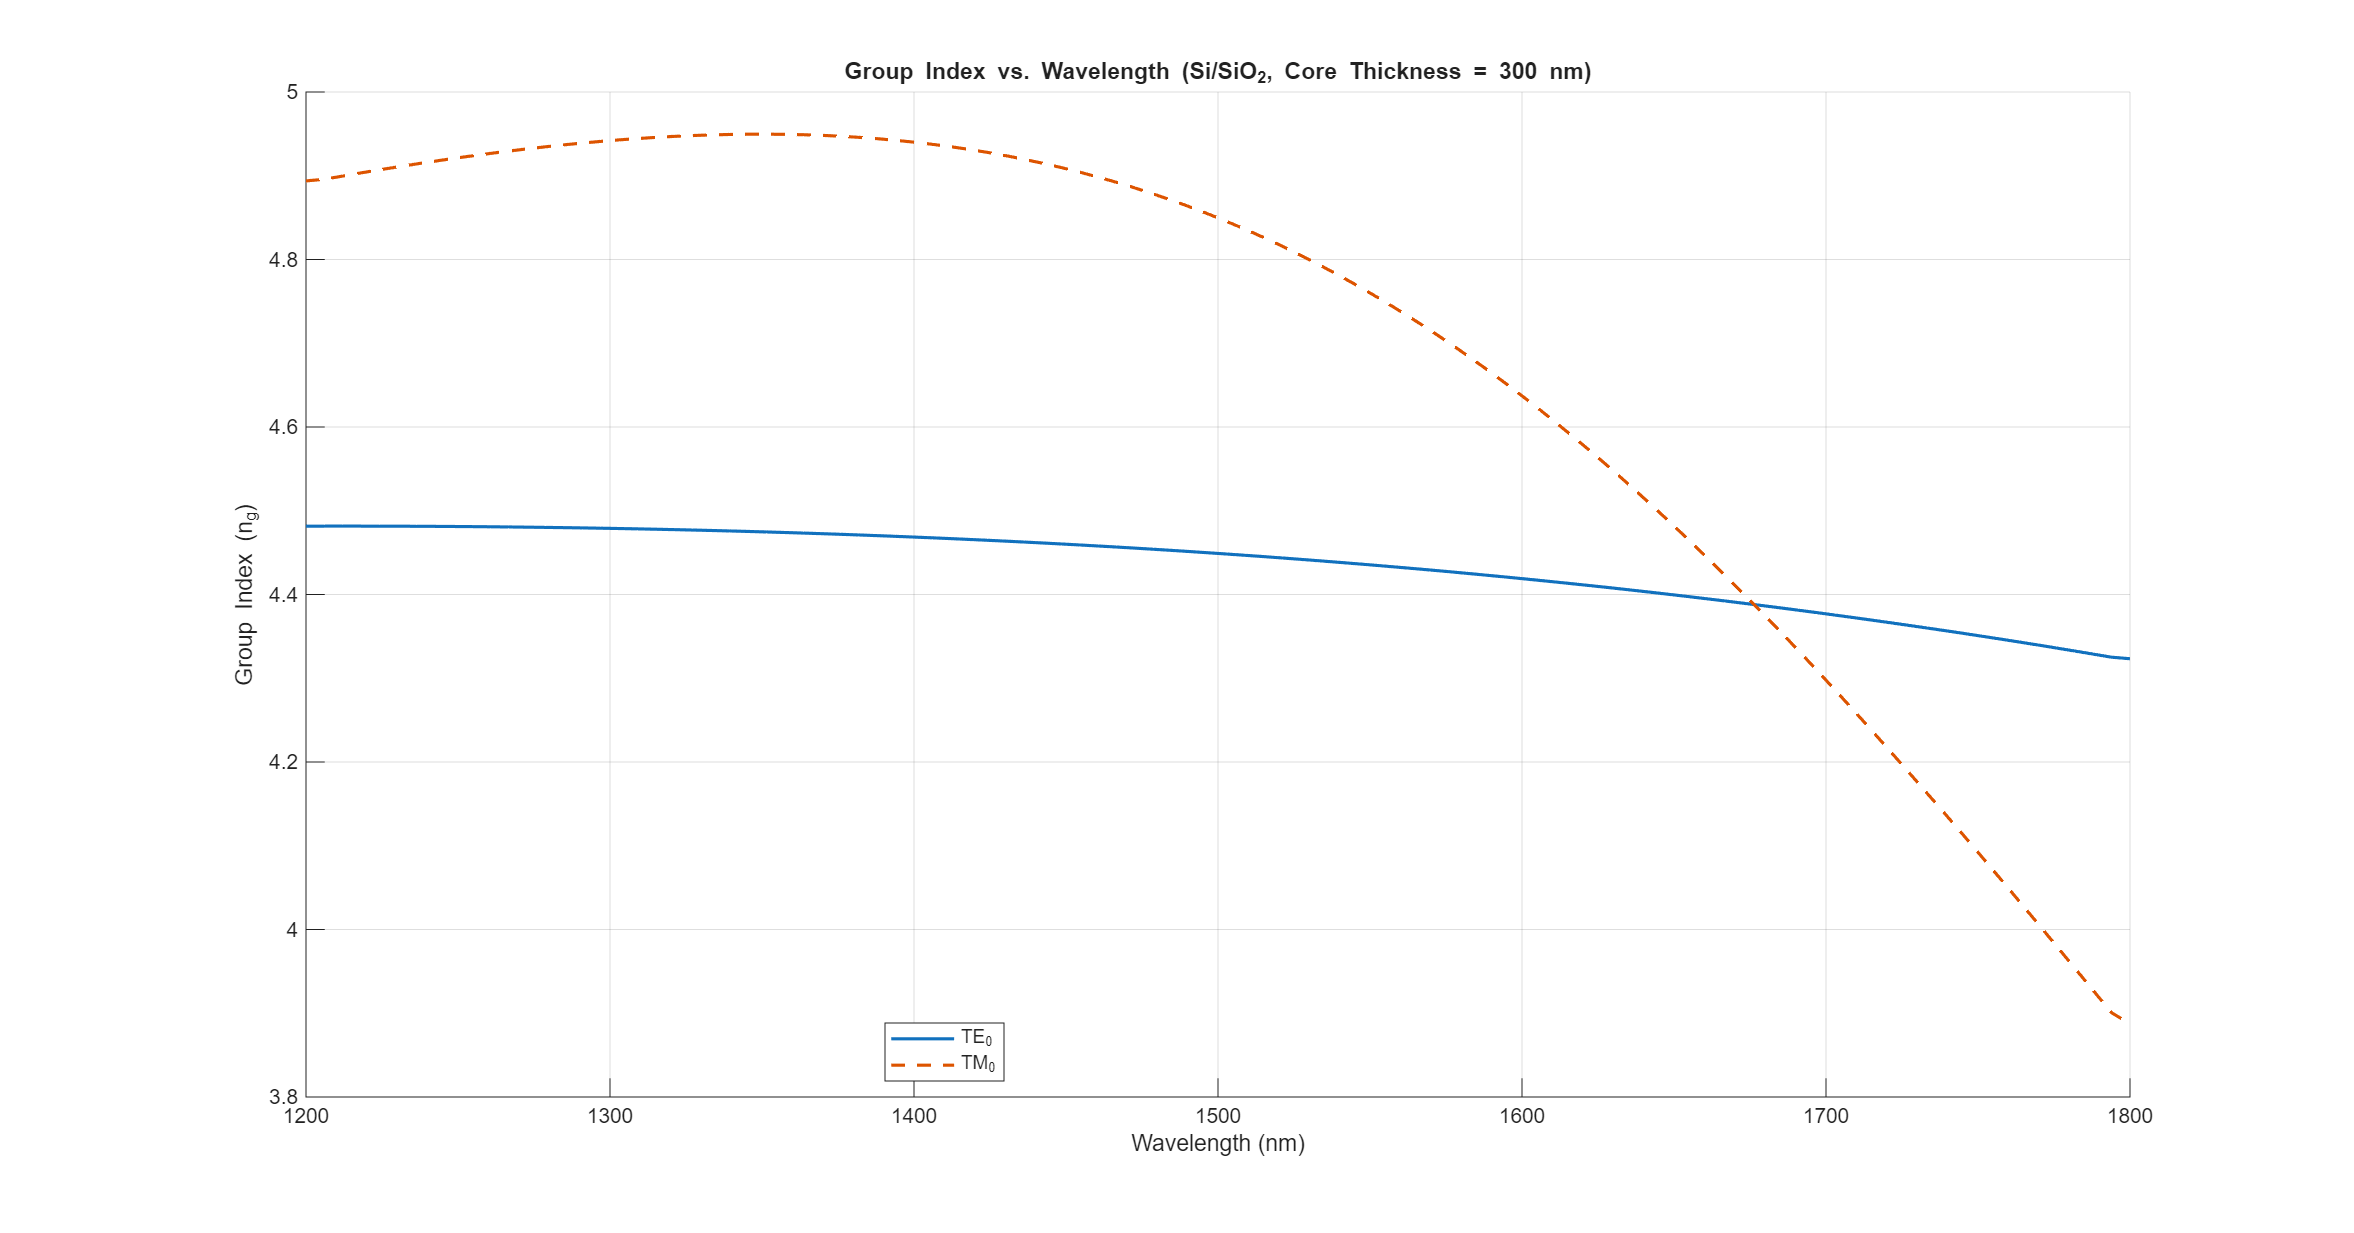
\includegraphics[width=0.8\textwidth]{task1/group_index_TE0_TM0_vs_wavelength_d300nm.png}
    \caption{Group index ($n_g$) vs. wavelength for TE$_0$ and TM$_0$ modes in an Si/SiO$_2$ waveguide with a 300~nm core thickness.}
    \label{fig:group_index_TE0_TM0_vs_wavelength}
\end{figure}

\subsection{Other SPW platforms}
To understand the impact of material choice, the SOI waveguide was compared to platforms using other core materials, all with an SiO$_2$ cladding:

\begin{itemize}
    \item Si\autocite{aspnesDielectricFunctionsOptical1983}
    \item Si$_3$N$_4$\autocite{lukeBroadbandMidinfraredFrequency2015}
    \item LiNbO$_3$\autocite{zelmonInfraredCorrectedSellmeier1997} (congruently grown)
    \item GaAs\autocite{adachiOpticalDispersionRelations1989}
\end{itemize}

Refractive indices at all swept wavelengths were interpolated in the \texttt{sb4.get\_n} function from \url{https://refractiveindex.info}~\autocite{polyanskiyRefractiveindexinfoDatabaseOptical2024}.

Note that, particularly for GaAs, being a III-V material, a much more common cladding is AlGaAs to achieve perfect lattice matching, but SiO$_2$ can also be used and is common in hybrid integration / wafer bonding where strong confinement is required.

\paragraph{Mode Count Comparison}
Figure~\ref{fig:modes_vs_thickness_materials_1550nm} compares the number of supported modes versus core thickness for these materials at $\lambda = 1550$~nm. Materials with a higher refractive index contrast with the cladding (e.g., Si, GaAs) generally support more modes for a given thickness than those with lower contrast (e.g., Si$_3$N$_4$, LiNbO$_3$). For instance, Si$_3$N$_4$ has a lower core index than Si, leading to a smaller index contrast with SiO$_2$ but potentially supporting more modes than LiNbO$_3$ if the LiNbO$_3$ index contrast is not as favorable or its specific dispersion limits mode count. The exact behavior depends on the precise refractive indices at the operating wavelength.

\begin{figure}[h!]
    \centering
    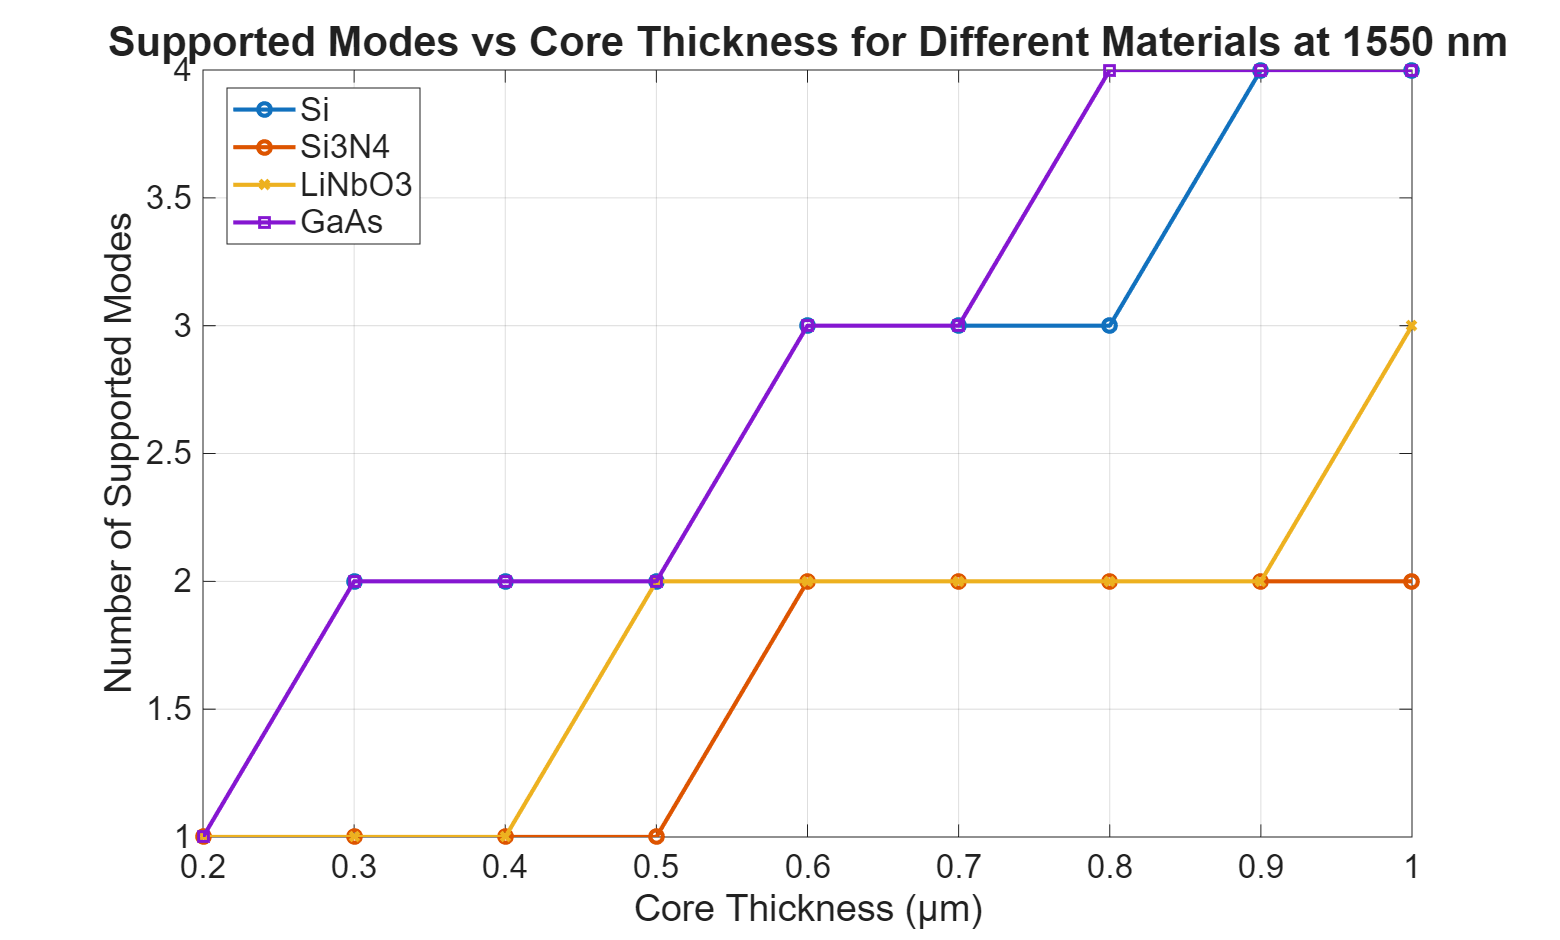
\includegraphics[width=0.8\textwidth]{task1/modes_vs_thickness_materials_1550nm.png}
    \caption{Number of supported modes vs. core thickness for different core materials (Si, Si$_3$N$_4$, LiNbO$_3$, GaAs) with SiO$_2$ cladding at $\lambda = 1550$~nm.}
    \label{fig:modes_vs_thickness_materials_1550nm}
\end{figure}

\paragraph{Critical Thickness for Multimode Operation}
The critical core thickness for the onset of multimode operation (i.e., cutoff of the $m=1$ mode) is plotted against wavelength for the different core materials in Figure~\ref{fig:critical_thickness_multimode_vs_wavelength_materials}. Materials with higher index contrast (like Si) allow for single-mode operation up to smaller thicknesses compared to lower-contrast materials. This plot highlights design trade-offs for achieving single-mode waveguides across different wavelengths and material systems.

\begin{figure}[h!]
    \centering
    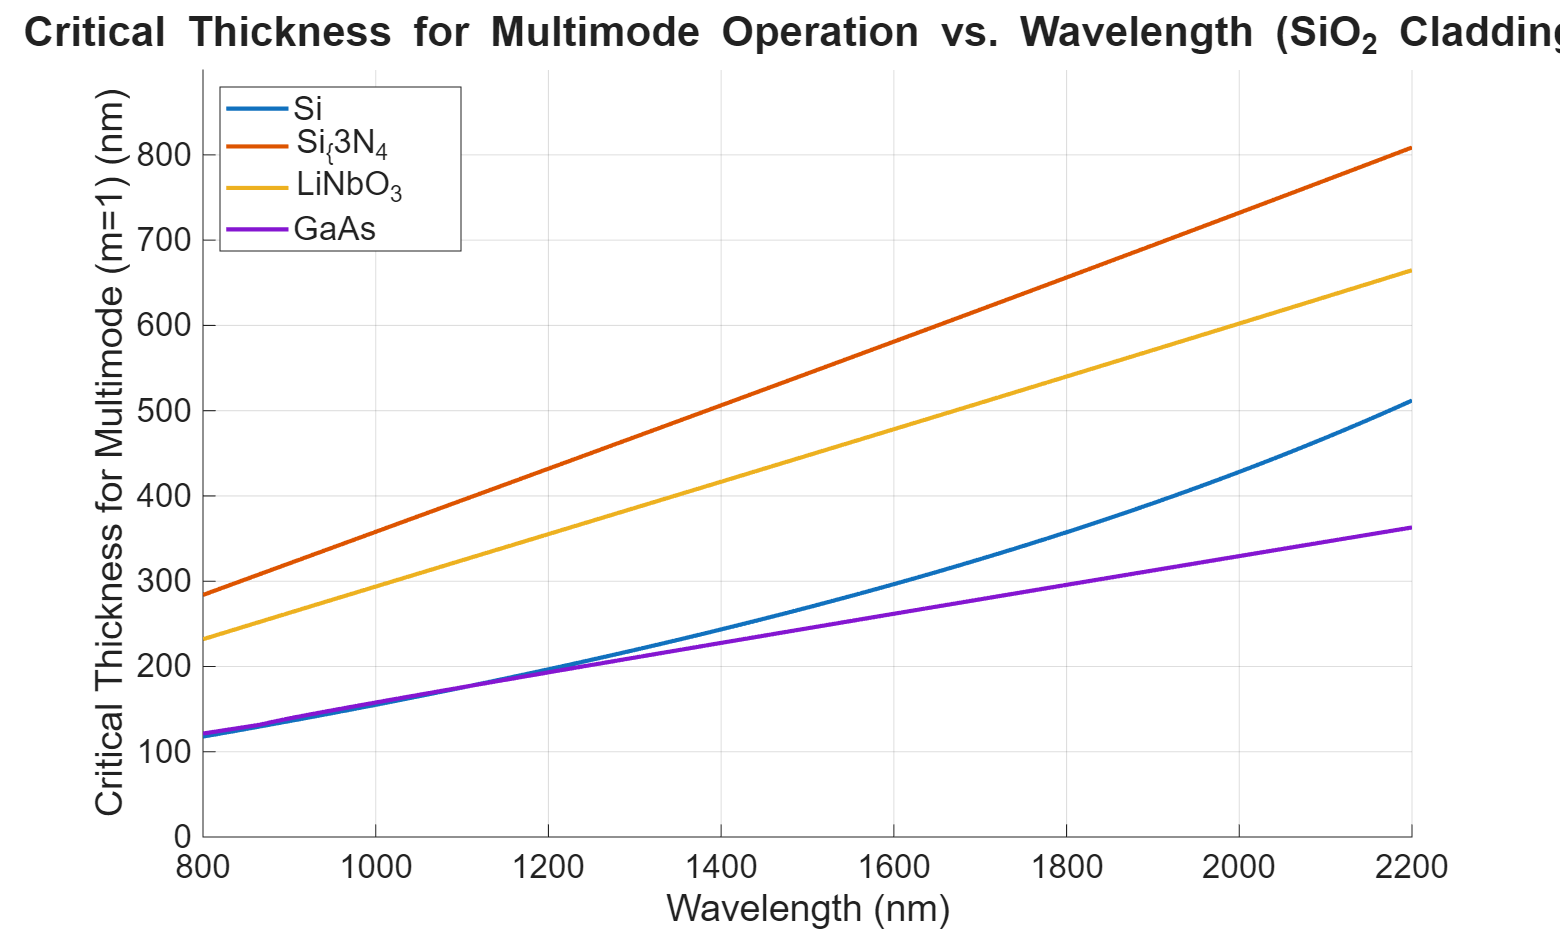
\includegraphics[width=0.8\textwidth]{task1/critical_thickness_multimode_vs_wavelength_materials.png}
    \caption{Critical core thickness for multimode operation ($m=1$ mode cutoff) vs. wavelength for different core materials with SiO$_2$ cladding.}
    \label{fig:critical_thickness_multimode_vs_wavelength_materials}
\end{figure}

\paragraph{Waveguide Birefringence}
Waveguide birefringence, $\Delta n = n_{\text{eff,TE}_0} - n_{\text{eff,TM}_0}$, arises from the different boundary conditions experienced by TE and TM modes. Figure~\ref{fig:birefringence_vs_thickness_materials_1550nm} shows the birefringence for the fundamental modes as a function of core thickness at $\lambda = 1550$~nm for the selected materials. Birefringence is strongly dependent on core thickness and material properties. High index contrast materials like Si and GaAs can exhibit significant birefringence, which can be tuned by waveguide geometry. While high birefringence is often desirable for applications like polarization control, it can also lead to polarization-dependent losses, pulse broadening and mode splitting.

\begin{figure}[h!]
    \centering
    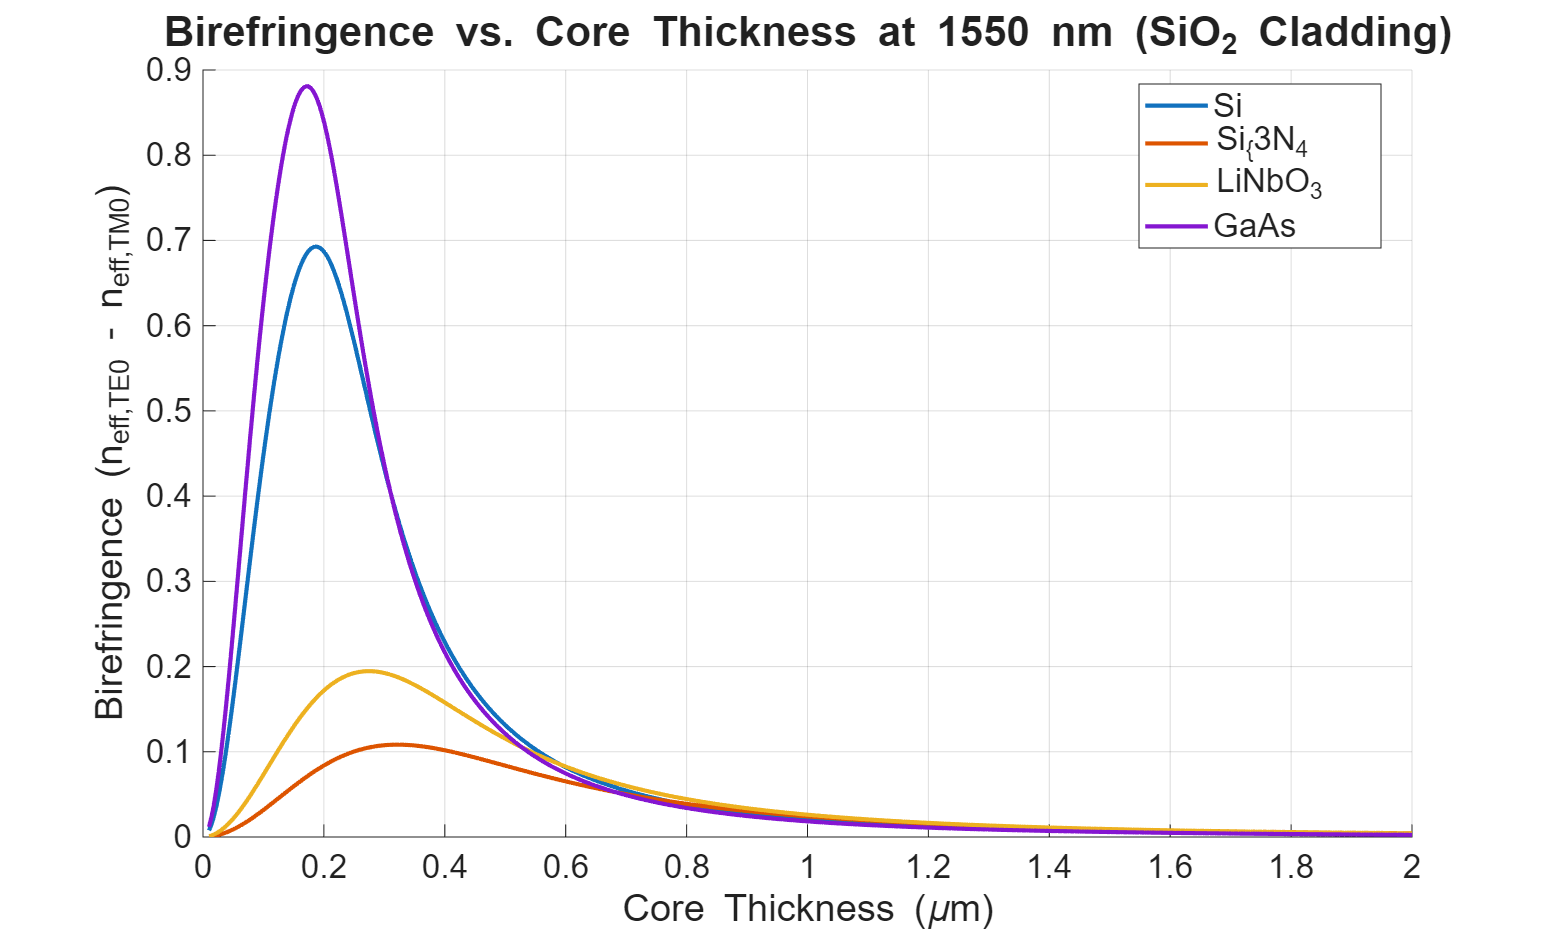
\includegraphics[width=0.8\textwidth]{task1/birefringence_vs_thickness_materials_1550nm.png}
    \caption{Birefringence ($n_{\text{eff,TE}_0} - n_{\text{eff,TM}_0}$) vs. core thickness for different core materials with SiO$_2$ cladding at $\lambda = 1550$~nm.}
    \label{fig:birefringence_vs_thickness_materials_1550nm}
\end{figure}

\paragraph{Note on Material Absorption}
It is important to note that the preceding analyses primarily utilize the real part of the materials' refractive indices. In practice, material absorption (represented by the imaginary part of the refractive index) leads to propagation losses. While this absorption can slightly perturb the real part of the effective index, its main impact is on signal attenuation. For instance, silicon exhibits higher intrinsic absorption at shorter wavelengths (e.g., < 1.1~{\textmu}m) and can also suffer from free-carrier absorption depending on doping. Materials like Si$_3$N$_4$ are often chosen for applications requiring lower loss, despite their lower index contrast. The above calculations are therefore an idealized comparison based on waveguiding principles governed by real refractive indices, and practical device performance would also depend heavily on these loss characteristics. However, for integrated photonics, the length scale is typically small enough that our analysis is a sufficient approximation.

\printbibliography

\end{document}